%%% Template para anotações de aula
%%% Feito por Daniel Campos com base no template de Willian Chamma que fez com base no template de  Mikhail Klassen



\documentclass[12pt,a4paper, brazil]{article}

%%%%%%% INFORMAÇÕES DO CABEÇALHO
\newcommand{\workingDate}{\textsc{\selectlanguage{portuguese}\today}}
\newcommand{\userName}{utad79835}
\newcommand{\institution}{Universidade Aberta}
\usepackage{researchdiary_png}
\usepackage{listings}


\begin{document}

\begin{center}
{\textbf {\huge Proposta de Projeto do Semestre}}\\[5mm]
{\large Ezequiel França dos Santos} \\[5mm]
\today\\[5mm] %% se quiser colocar data
\end{center}


\section{Resumo}

Proposta de um Activity Provider na arquitetura Inven!RA. Um Activity Provider baseado em geolocalização onde o professor consegue saber onde foi feita a atividade, e posteriormente até montar um mapa com todos. Pode ser utilizada para criar missões de observação de obras de arte, esculturas, ou quaisquer outros pontos de interesse.

\section{Requisitos do Projeto}

A concepção e desenvolvimento de um desses módulos, para integração na arquitetura Inven!RA.\cite{https://doi.org/10.34627/rcc.v16i0.268}


\begin{figure}[ht]
    \centering
    \caption{Diagrama de Sequencia.}
    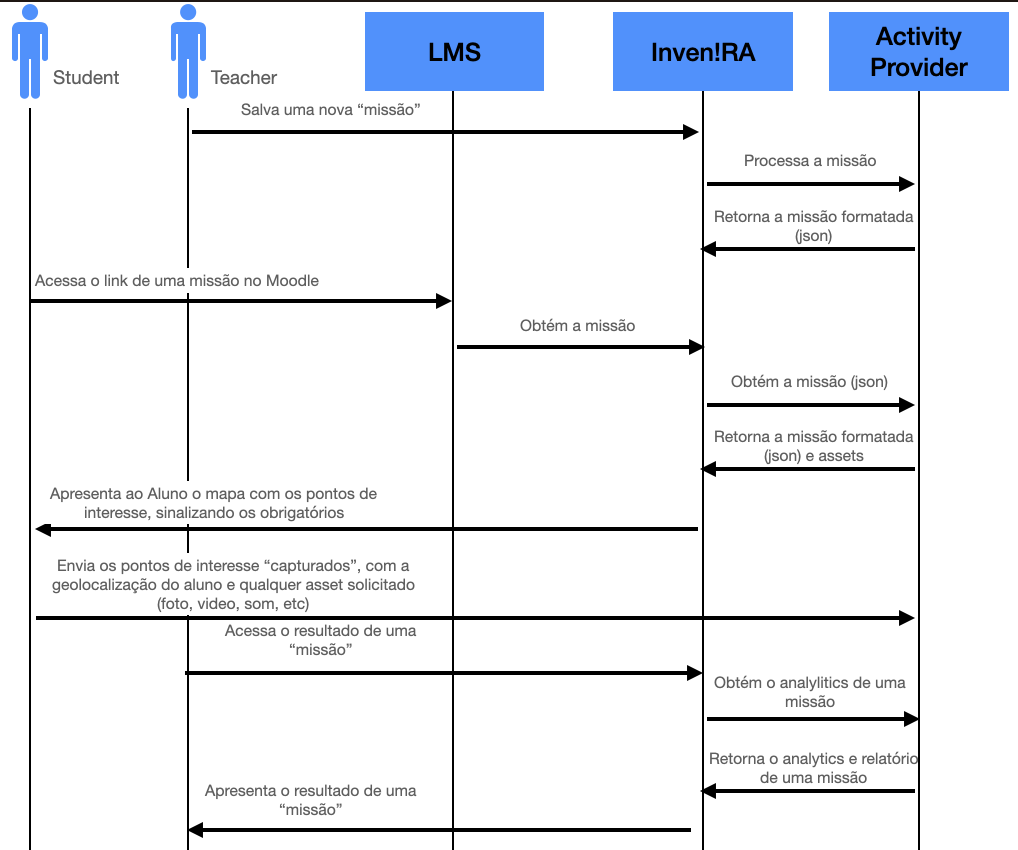
\includegraphics[width=0.85\textwidth]{diagrama_sequencia.png}
    \label{fig:exemplo}
\end{figure}

\section{JSON}

Desenvolvimento de um serviço baseado em geolocalização que processe os dados entre o LMS e a Inven!RA com a estrutura básica seguinte:

\begin{figure}[ht]
    \centering
    \caption{Representaçao do Modelo}
    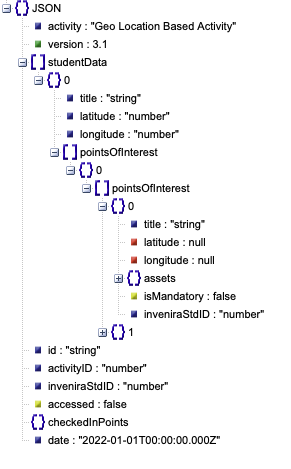
\includegraphics[width=0.67\textwidth]{json.png}
    \label{fig:exemplo}
\end{figure}

\pagebreak
\begin{lstlisting}[language=javascript]

{
  "activity": "Geo Location Based Activity",
  "studentData": [
    {
      "title": "string",
      "latitude": "number",
      "longitude": "number",
      "pointsOfInterest": [
        {
          "pointsOfInterest": [
            {
              "title": "string",
              "latitude": null,
              "longitude": null,
              "assets": {
                "assets": [
                  {
                    "imageURL": "null",
                    "videoURL": "null",
                    "soundURL": "null"
                  }
                ]
              },
              "isMandatory": false,
              "inveniraStdID": "number"
            }
          ]
        }
      ]
    }
  ],
  "id": "string",
  "activityID": "number",
  "accessed": false,
  "checkedInPoints": {},
  "date": "2022-01-01T00:00:00.000Z"
}

\end{lstlisting}

%%% as referências devem estar em formato bibTeX no arquivo referencias.bib
\printbibliography

\end{document}